\documentclass{article}
\usepackage[utf8]{inputenc}
\textheight = 25cm 
\textwidth = 16cm
\topmargin = -3.0cm 
\oddsidemargin = 1cm
\usepackage{hyperref}
\hypersetup{
    colorlinks=true,
    linkcolor=blue,
    filecolor=blue,
    citecolor=black,      
    urlcolor=blue,
    }

\usepackage{float}
\usepackage{graphicx}

\usepackage{gensymb}

\usepackage{amsmath}
\DeclareMathOperator*{\argmax}{argmax} % thin space, limits 
\usepackage{amssymb}
\usepackage{amsfonts}
\usepackage{mathtools, xparse}
\usepackage[shortlabels]{enumitem}

\usepackage[many]{tcolorbox}
\usepackage{lipsum}
\usepackage{amssymb}

\title{Reinforcement Learning}
\author{Cerritos Lira, Carlos}
\date{23 de junio del 2020}

\newcommand{\pr}[1]{\left(#1\right)}
\newcommand{\pt}[2]{\dfrac{\partial #1}{\partial #2}}

\begin{document}
\maketitle
\section*{Markov Decision Process}
\begin{figure}[H]
    \centering
    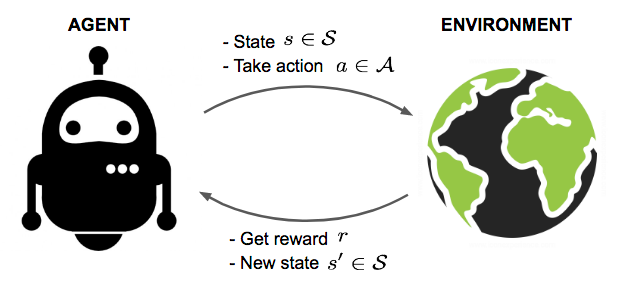
\includegraphics[scale=0.5]{images/mdp.png}
\end{figure}
\subsection*{Setup}
\begin{align*}
    R(s,a) &= \text{ Reward of taking action $a$ at state $s$} \\
    T(s,a,s') &= P(s' \mid s,a) \text{ Probability of getting to $s'$ given that we were in state $s$ and took aciton $a$} \\
    \pi(s) &= \text{ Policy, the action that we should take given that we are in state $s$} \\
    U^\pi(s) &= \text{ Utility, how good is a state}
\end{align*}
\subsection*{Bellman equation}
Given a policy $\pi$, we measure how good a state is by taking the expected sum of ininite discounted rewards.
\begin{align*}
    U^\pi(s) &= E[\sum_{t=0}^\infty \gamma^t R(s_t) \mid \pi, s_0=s] \\
    U^\pi(s) &= E[R(s) + \gamma \sum_{t=0}^\infty \gamma^tR(s_t) \mid \pi, s_0=S'], \quad P_{S'}(s')=T(s,\pi(a),s') \\
    U^\pi(s) &= R(s) + \gamma \sum_{s'} T(s,\pi(s),s')U(s') \\
    \pi^*(s) &= \argmax_{a} \sum_{s'} T(s,a,s')U(s') \\
    U(s) &= R(s) + \gamma \max_{a} \sum_{s'} T(s,a,s')U(s') 
\end{align*}
\subsection*{Value interation}
The straight forward way of updating $U_T$ is:
\begin{align*}
    U_T(s) &= R(s)+\gamma \max_{a} \sum_{s'} T(s,a,s')U_{T-1}(s')
\end{align*}
define the Bellman operator such that:
\begin{align*}
    U_T &= BU_{T-1}
\end{align*}
since the Bellman operator is a contraction and $U$ is a fixed point this method should converge 
to $U$. 
\subsection*{Q-learning}
\begin{align*}
    Q(s,a) 
    &= R(s,a)+\gamma \sum_{s'}T(s,a,s')\max_{a'}Q(s',a') \\
    Q_T(s_{t-1},a_{t-1}) &= Q_{T-1}(s_{t-1},a_{t-1}) + \alpha_T(r_t + \gamma \max_{a'}Q_{T-1}(s_{t-1},a')+Q_{T-1}(s_{t-1},a_{t-1}))
\end{align*}


\end{document}